\section{Db2 Graph}
\label{db2graph}

Im Rahmen dieses Kapitels wird IBM Db2 Graph genauer beschrieben. Im Zuge dessen werden der Ansatz, der Aufbau, die Funktionsweise und die bereits bekannten Einschränkungen von Db2 Graph erläutert. Außerdem werden die verschiedenen Optimierungsmechanismen von Db2 Graph erörtert und die Unterschiede zwischen den Versionen von Db2 Graph behandelt, die im Rahmen der Arbeit eine Rolle spielen. Abschließend werden die wichtigsten Details zu Db2 Graph nochmals kurz zusammengefasst.

\subsection{Ansatz}
\label{db2graph:ansatz}
Db2 Graph wurde mit dem Ziel entwickelt, Informationen mittels Graph-Queries aus einer relationalen Db2-Datenbank abfragen zu können \cite{vldb_tian, sigmod_tian}. So wurde Db2 Graph als eine Grapherweiterung für Db2 konzipiert. Der Einsatz von Db2 Graph setzt dabei eine aktive Instanz von Db2 voraus \cite{vldb_tian, sigmod_tian}. Diese hält die Informationen, auf die Db2 Graph Zugriff hat in relationaler Form \cite{vldb_tian, sigmod_tian}. Dabei müssen die Daten nicht für die Einbindung in Db2 Graph angepasst oder umformatiert werden \cite{vldb_tian, sigmod_tian}.

\begin{figure}[!ht]
	\usetikzlibrary{shapes.arrows}
    \centering
	\begin{tikzpicture}[
		nodestyle/.style={draw, minimum height=15mm, minimum width=25mm},
		databasenode/.style={cylinder, draw, thick, shape border rotate=90, shape aspect=.5, minimum height=17mm, minimum width=25mm, align=center, outer sep=-0.5\pgflinewidth, yshift=-2mm},
		arrowstyle/.style={draw, double arrow, minimum width=0.7cm, minimum height=2cm, double arrow head extend=0.2cm}
		]
		\node[nodestyle] (client) at (0, 0) {Client};
		\node[nodestyle] (graph) at (5, 0) {DB2 Graph};
		\node[databasenode] (db2) at (10, 0) {Db2};
		\node[arrowstyle] at (2.5, 0) {};
		\node[arrowstyle] at (7.5, 0) {};
	\end{tikzpicture}
    \vspace{0.1em}
    \caption{Rolle Db2 Graph}
    \label{fig:db2graph_system}
\end{figure}

Wie in \autoref{fig:db2graph_system} erkennbar, fungiert Db2 Graph aus architektonischer Sicht als eine Art Proxy-Anwendung für Db2. Dabei übersetzt sie die von einem Client gesendeten Gremlin-Graph-Queries in SQL-An\-wei\-sung\-en \cite{vldb_tian, sigmod_tian}. Diese werden anschließend an eine Db2-Instanz weitergeleitet \cite{vldb_tian, sigmod_tian}. 

Db2 Graph und Db2 erfüllen somit gemeinsam die Rolle einer Read-Only-Graph\-daten\-bank. Db2 Graph vereint dabei Elemente von Graphdatenbanksystemen und relationalen Datenbanksystemen. So ist es möglich, Graphanfragen an ein System zu stellen, das die Daten in relationaler Form speichert \cite{vldb_tian, sigmod_tian}. Dadurch bringt Db2 Graph das Abfragen von Elementen einer Graphstruktur mit einer relationalen Datenhaltung zusammen. 

\subsection{Aufbau}
Wie in \autoref{fig:db2graph_aufbau} beschrieben, handelt es sich bei Db2 Graph um eine modular aufgebaute Anwendung. Die Anwendung besteht dabei aus fünf größeren Komponenten. Diese fünf Komponenten übernehmen dabei die folgenden Rollen und Aufgaben: 

\begin{itemize}
    \item \textit{TinkerPop-Stack}\\Stellt das Grundgerüst für Db2 Graph dar. Er parst eingehende Gremlin-Queries und erstellt auf Basis dessen einen Query-Plan bzw. Abfrage-Plan \cite{vldb_tian}. Dabei interagiert er über API-Aufrufe mit den anderen Modulen \cite{vldb_tian}.
    \item \textit{Topology}\\Beinhaltet die Funktionalität für das Mapping von Tabellen aus einer relationalen Datenbank auf eine Graphstruktur \cite{vldb_tian, sigmod_tian}.
    \item \textit{Graph Structure}\\Hierbei handelt es sich um eine eigene Implementierung einer Graphstruktur, auf deren Basis TinkerPop arbeitet \cite{vldb_tian}. Eine Implementierung dieser Struktur wird benötigt, um den vom TinkerPop-Stack erstellten Query-Plan durchzuführen \cite{sigmod_tian}. 
    \item \textit{SQL-Dialect}\\Diese Komponente stellt die Funktionalität für die Erzeugung von Db2-kompatiblen SQL-Anweisungen bereit \cite{sigmod_tian}.
    \item \textit{Traversal-Strategy}\\Dieses Modul stellt dem TinkerPop-Stack optimierte Traversal-Strategies zur Verfügung. Diese werden eingesetzt, um einen vom TinkerPop-Stack aufgestellten Query-Plan zu optimieren, bevor dieser ausgeführt wird \cite{sigmod_tian}.  
\end{itemize}

\begin{figure}[!ht]
    \centering
    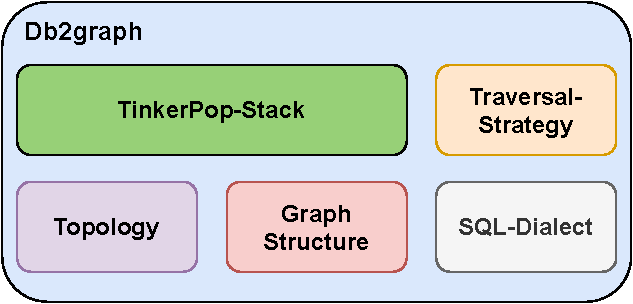
\includegraphics[width=\textwidth]{images/db2graph_components.pdf}
    \caption{Aufbau von Db2 Graph}
    \label{fig:db2graph_aufbau}
    \vspace{0.5em}
    \textit{Der hier gezeigte Aufbau von Db2 Graph orientiert sich an der Beschreibung der System-Architektur von} \citeAYY{vldb_tian}{sigmod_tian}\textit{.}
\end{figure}

Der TinkerPop-Stack stellt somit den Kern von Db2 Graph dar. Die Topology-, Graph-Structure- und SQL-Dialect-Komponente abstrahieren die Db2 Graph spezifische Funktionalität, auf die der TinkerPop-Stack zugreifen kann \cite{sigmod_tian}. Zusätzlich dazu stellt das Traversal-Strategy-Modul dem TinkerPop-Stack, optimierte Traversal-Strategies bereit \cite{sigmod_tian}. Diese helfen dem TinkerPop-Stack dabei, die Performance von Query-Plans zu verbessern \cite{sigmod_tian}.

\subsection{Funktionsweise}
\label{db2graph:funktionsweise}
Um die Funktionsweise von Db2 Graph genauer zu erläutern, wird in diesem Abschnitt die Funktionsweise aus verschiedenen Perspektiven erläutert. Im Rahmen der ersten externen Perspektive wird detailliert darauf eingegangen, wie die Anfrage eines Clients in Db2 Graph und Db2 verarbeitet wird. Der Fokus liegt hierbei auf der Kommunikation zwischen den Anwendungen. Bei der zweiten Perspektive handelt es sich hingegen um die Db2 Graph interne Perspektive. Im Zuge dessen wird beschrieben, wie eine Gremlin-Abfrage von einer Db2-Graph-Anwendung intern verarbeitet wird. 

Im Anschluss an diese beiden Perspektiven werden der Begriff und die Funktionsweise des Mappings in Db2 Graph genauer erläutert. Schließlich spielen die damit in Verbindung stehenden Topologie-Informationen eine wichtige Rolle für die Verarbeitung von Anfragen.

\subsubsection{Extern}
Im Rahmen dieses Unterabschnitts wird darauf eingegangen, wie die Verarbeitung einer Anfrage (Gremlin-Query) im Kontext der voneinander entkoppelten Bestandteile Client(-Anwendung), Db2 Graph und Db2 erfolgt. Der Ablauf der Verarbeitung kann dabei in die folgenden Schritte unterteilt werden: 
\begin{enumerate}
    \item Ein Client sendet eine Gremlin-Query an Db2 Graph. 
    \item Db2 Graph wandelt die Gremlin-Query in SQL-Statements um. 
    \item Db2 Graph sendet die erzeugten SQL-Statements an Db2.
    \item Db2 verarbeitet die SQL-Statements.
    \item Db2 leitet die Ergebnisse an Db2 Graph weiter.
    \item Db2 Graph bereitet die von Db2 empfangenen Ergebnisse für den Client auf. 
    \item Db2 Graph übermittelt die Ergebnisse an den Client.
\end{enumerate}

Die soeben beschriebenen Schritte des Ablaufs können dabei den in der \autoref{fig:db2graph_processing} aufgeführten Schritten zugeordnet werden. Die in \autoref{fig:db2graph_processing} als grün gekennzeichneten Pfeile markieren dabei die Schritte, bei denen die Anfrage in Form einer Gremlin-Query oder SQL-Anfragen weitergeleitet oder verarbeitet wird. Die Pfeile, welche in \autoref{fig:db2graph_processing} lila gefärbt sind, heben die Schritte hervor, in denen die abgefragten Daten transformiert oder weitergeleitet werden.

\begin{figure}[ht]
    \centering
    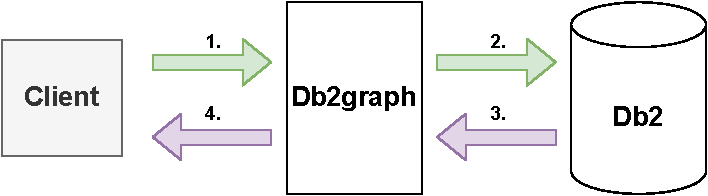
\includegraphics[width=\textwidth]{images/db2graph_processing.pdf}
    \caption{Externe Verarbeitung Db2 Graph}
    \label{fig:db2graph_processing}
    \vspace{1em}
    \textit{Die dargestellten Abläufe basieren hierbei unter anderem auf den von} \citeAYY{vldb_tian}{sigmod_tian} \textit{beschriebenen Abläufen der Verarbeitung. Darüber hinaus wurden auch einige kleinere Details aus der} \citeAY{tinkerpop_2020} \textit{bezogen.} 
\end{figure}

\subsubsection{Intern}
Im Rahmen dieses Unterabschnitts wird dargelegt, wie eine von Db2 Graph empfangene Gremlin-Query intern verarbeitet wird. Der Ablauf kann dabei in die folgenden Schritte gegliedert werden: 

\begin{enumerate}
    \item Ein Client baut eine Verbindung auf und sendet eine Gremlin-Query an Db2 Graph.
    \item Der TinkerPop-Stack lädt Informationen über die Beschaffenheit des in der Gremlin-Query enthaltenen Zielgraphen aus der Topology-Komponente \cite{vldb_tian,sigmod_tian, yt_tian}.
    \item Der TinkerPop-Stack erstellt auf Basis der Gremlin-Query und der Topologieinformationen einen logischen Query-Plan \cite{vldb_tian,sigmod_tian, yt_tian}. 
    \item Der TinkerPop-Stack nutzt das Traversal-Strategy-Modul, um den logischen Query-Plan zu optimieren \cite{vldb_tian,sigmod_tian, yt_tian}. Wie und welche Optimierungen an dieser Stelle angewandt werden, wird in \autoref{db2graph:optimierung} genauer erläutert.
    \item Der TinkerPop-Stack wandelt den optimierten, logischen Query-Plan in einen physikalischen Query-Plan um \cite{vldb_tian,sigmod_tian, yt_tian}. 
    \item Bei der Ausführung der Steps im physikalischen Query-Plan werden API-Zugriffe auf die Graph-Structure-Komponente durchgeführt \cite{vldb_tian,sigmod_tian, yt_tian}. Um die für diese Zugriffe benötigten Informationen zu beschaffen, lädt die Graph-Structure-Komponente Informationen aus dem Topology-Modul und nutzt die SQL-Dialect-Komponente für die Erzeugung von SQL-Statements \cite{vldb_tian,sigmod_tian, yt_tian}. Bei diesem Schritt können ebenfalls Optimierungen angewandt werden. Diese werden in \autoref{db2graph:optimierung} detailliert beschrieben.
    \item Die von der Graph-Structure-Komponente erzeugten SQL-Statements werden an eine Db2-Instanz gesendet und von dieser verarbeitet \cite{vldb_tian,sigmod_tian, yt_tian}.
    \item Die daraufhin von Db2 erhaltenen und zurückgesendeten Ergebnisse werden von der Graph-Structure-Komponente verarbeitet \cite{yt_tian}. 
    \item Die Graph-Komponente nutzt die verarbeiteten Ergebnisse, um die API-Aufrufe des TinkerPop-Stacks zu beantworten \cite{vldb_tian,sigmod_tian, yt_tian}.
    \item Nach der Durchführung des physikalischen Query-Plans -- inklusive der API-Aufrufe auf die Graph-Structure-Komponente -- werden die Ergebnisse vom TinkerPop-Stack an den Client übermittelt \cite{vldb_tian,sigmod_tian,yt_tian}.
\end{enumerate}

Die Schritte 1. bis 7. der internen Verarbeitung von Queries werden dabei zum besseren Verständnis in \autoref{fig:db2graph_intern_processing} nochmals dargestellt.

\begin{figure}[ht]
    \centering
    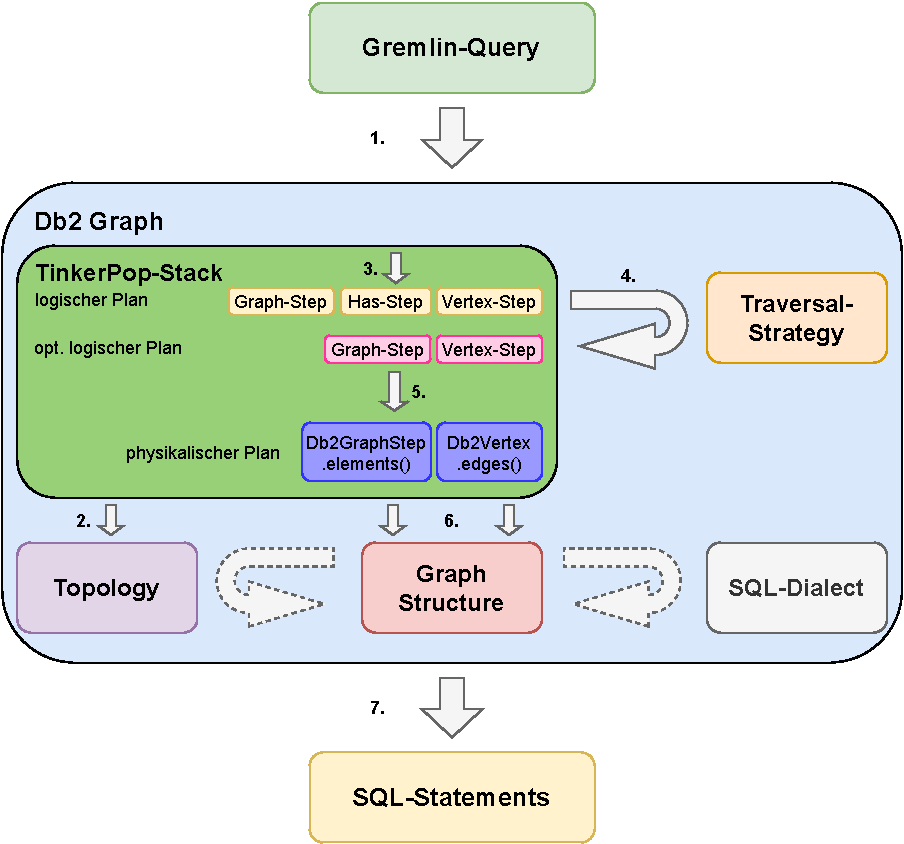
\includegraphics[width=\textwidth]{images/db2graph_intern_processing.pdf}
    \caption{Interne Verarbeitung Db2 Graph}
    \label{fig:db2graph_intern_processing}
    \vspace{1em}
    \textit{Die in der Abbildung dargestellten Abläufe basieren auf den von} \citeAYY{vldb_tian}{sigmod_tian} und \citeAY{yt_tian} \textit{beschriebenen Abläufen.} 
\end{figure}

\subsubsection{Mapping}
Bei dem sogenannten Mapping handelt es sich um den Db2 Graph-internen Prozess beziehungsweise Technik, bei dem eine Graphstruktur relationalen Daten übergestülpt wird beziehungsweise diese überlagert. Der Prozess kann auch als Graph-Overlaying bezeichnet werden. Vereinfacht ausgedrückt, handelt es sich dabei um die Spezifikation der Topologie des von Db2 Graph abgebildeten Graphen. In dieser Spezifikation wird festgelegt, welche Tabellen und Spalten auf welche Graph-Elemente (Knoten und Kanten) gemappt werden. 

Für die Bereitstellung und Verarbeitung des Mapping in Db2 Graph ist hierbei die Topology-Komponente zuständig. Das Mapping wird dabei in einer als Graph-Overlay-Konfiguration bezeichneten Datei festgehalten.  

Um das Mapping von relationalen Strukturen auf Graphstrukturen durchzuführen, werden den Tabellen einer Db2-Datenbank verschiedene Rollen zugewiesen. Dabei sind die zwei folgenden Rollen verfügbar:
\begin{itemize}
    \item \textit{Vertex-Tabelle}\\Die Zeilen einer Tabelle werden als Knoten auf einen Graph gemappt \cite{sigmod_tian, yt_tian}.
    \item \textit{Edge-Tabelle}\\Die Zeilen dieser Tabelle werden als Kanten auf einen Graph gemappt \cite{sigmod_tian, yt_tian}.
\end{itemize}

Um Verbindungen zwischen Kanten und Knoten herzustellen, verfügt eine Vertex-Tabelle über eine Vertex-ID (\texttt{\acs{vid}}). Diese \texttt{\acs{vid}} kann als eine Art Primärschlüssel betrachtet werden. Die \texttt{\acs{vid}} setzt sich dabei aus einer oder mehreren Spalten einer relationalen Tabelle und einem Prefix zusammen \cite{sigmod_tian, yt_tian}, siehe \texttt{prefix} und \texttt{id\_cols} Zeile 5 -- 6 in \autoref{src:mapping_example}. Ihr Zweck ist es dabei, immer einen einzigen bestimmten Knoten über den Wert der \texttt{\acs{vid}} identifizieren zu können \cite{sigmod_tian, yt_tian}. 

Auf Basis dieser \texttt{\acs{vid}} (Zeile 4 -- 7 \autoref{src:mapping_example}) setzt bei dem Mapping auch die Edge-Tabelle auf. So ist es notwendig, den Start- und Zielknoten einer Kante in der Edge-Tabelle anzugeben. Dafür muss bei der Referenzierung eines Startknotens in der Graph-Overlay-Konfiguration die Tabellen-ID der Vertex-Tabelle angegeben werden, die den Startknoten enthält. Dies geschieht in \autoref{src:mapping_example} durch \texttt{table\_id} und \texttt{src\_v\_tables} Zeile 8 und 23. Zusätzlich dazu müssen auch die Spalten in der Edge-Tabelle spezifiziert werden, anhand derer eine Zeile der Vertex-Tabelle referenziert wird, wie bei den \texttt{src\_v\_cols} in Zeile 21 \autoref{src:mapping_example}. Die Referenzierung eines Zielknotens funktioniert dabei ähnlich. Den einzigen Unterschied stellt dabei die Verwendung der Felder \texttt{dst\_v\_cols} und \texttt{dst\_v\_tables} (Zeile 22 und 24 des \autoref{src:mapping_example}) dar, statt \texttt{src\_v\_cols} und \texttt{src\_v\_tables}.

Wie in \autoref{src:mapping_example} erkennbar, lässt die Konfiguration auch weitere Anpassungen bezüglich des Mappings und der Graph-Topologie zu. So ist es beispielsweise möglich, die Labels für Knoten und Kanten auf Basis einer Vertex-Tabelle oder Edge-Tabelle zu definieren, siehe Zeile 15 und 43 \autoref{src:mapping_example}. Der Kern des Mappings spielt sich dabei aber wie zuvor beschrieben auf Basis der Parameter \texttt{\acs{vid}}, \texttt{table\_id}, \texttt{src\_v\_cols}, \texttt{dst\_v\_cols} sowie \texttt{src\_v\_tables} und \texttt{dst\_v\_tables} ab. Diese Werte bestimmten, wie die relationalen Daten auf einem Graph abgebildet werden.

\begin{lstlisting}[caption={Beispiel Ausschnitt Mapping Konfiguration},language=json,label=src:mapping_example]
{
    "v_tables": [
            {
            "vid": {
                "prefix": "LINKDB0.NODETABLE",
                "id_cols": ["ID"]
            },
            "table_id": "LINKDB0.NODETABLE",
            "table": {
                "schema_name": "LINKDB0",
                "table_name": "NODETABLE"
            },
            "label": {
                "fixed_label": true,
                "label": "NODETABLE"
            }
        }
    ],
    "e_tables": [
        {
            "src_v_cols": ["ID1"],
            "dst_v_cols": ["ID2"],
            "src_v_tables": ["LINKDB0.NODETABLE"],
            "dst_v_tables": ["LINKDB0.NODETABLE"],
            "eid": {
                "implicit_id": false,
                "id": {
                    "prefix": "LINKDB0.LINKTABLE",
                    "id_cols": [
                        "LINK_TYPE",
                        "ID1",
                        "ID2"
                    ]
                }
            },
            "table_id": "LINKDB0.LINKTABLE",
            "table": {
                "schema_name": "LINKDB0",
                "table_name": "LINKTABLE"
            },
            "label": {
                "fixed_label": true,
                "label": "LINKTABLE"
            }
        }
    ]
}
\end{lstlisting}

Abschließend zum Thema Mapping sollte auch darauf hingewiesen werden, dass nicht alle Tabellen einer Datenbank oder eines bestimmten Schemas auf einen Graphen gemappt werden müssen. Es ist vollkommen legitim, Tabellen im relationalen Modell keine Rolle als Vertex-Tabelle oder Edge-Tabelle zuzuweisen. Besonders, wenn die Daten im Kontext des Graphen nicht benötigt werden. 

\subsection{Fähigkeiten und Einschränkungen}
Im Rahmen dieses Kapitels werden die bekannten Fähigkeiten und Einschränkungen von Db2 Graph kurz zusammengefasst. Dies ist hier von besonderem Interesse, da es sich bei Db2 Graph in Kombination mit Db2 um eine Art hybrides Datenbankmanagementsystem handelt. Auf die besonderen Eigenschaften des Systems, die sich aus der Verbindung von relationalem und Graph-Datenbanksystem ergeben, wird hier ebenfalls eingegangen. 

Db2 Graph verfügt über die folgenden Fähigkeiten und Einschränkungen:

\begin{itemize}
    \item \textit{Read-Only-Queries}\\
    Db2 Graph verfügt über eine Art Read-Only-Implementierung von Apache TinkerPop, durch die es dazu in der Lage ist, nahezu alle lesenden Gremlin-Queries zu verarbeiten \cite{ibm_docs_limitiations}. Umgekehrt bedeutet dies allerdings auch, dass Db2 Graph nicht fähig ist, schreibende Gremlin-Queries zu verarbeiten.
    \item \textit{Optimierung}\\
    Db2 Graph verfügt über mehrere Mechanismen, um die Verarbeitung von empfangenen Gremlin-Queries zu optimieren. Diese Optimierungen werden in \autoref{db2graph:optimierung} genauer erläutert.
    \item \textit{Datentypen}\\
    Von Db2 Graph werden nur Datentypen unterstützt, die auch in Db2 vorhanden sind \cite{ibm_docs_limitiations}. Das bedeutet, dass lediglich diese Datentypen als Property-Type eines Knotens oder einer Kante eingesetzt werden können \cite{ibm_docs_limitiations}. Somit ist es auch nicht möglich, verschachtelte Datentypen -- wie z.B. in Neo4j -- als Property-Type zu nutzen. Schließlich werden diese nicht von Db2 Graph unterstützt.
    \item \textit{Festes Schema}\\
    Daten, die von Db2 Graph abgefragt werden können, verfügen über ein festes Schema. Dieses ergibt sich daraus, dass die Daten in einer Db2-Instanz (relational) gehalten und gespeichert werden \cite{sigmod_tian,vldb_tian,yt_tian}.
    \item \textit{GraphComputer}\\
    Der Gremlin-GraphComputer wird von Db2 Graph nicht unterstützt \cite{ibm_docs_limitiations}. Dadurch kann Db2 Graph diese Schnittstelle für komplexe Graph-Algorithmen nicht nutzen. Somit entgeht Db2 Graph die Fähigkeit, auf die bei dem GraphComputer vordefinierten Algorithmen \textit{PageRank}, \textit{PeerPressure} und \textit{ShortestPath} zuzugreifen.
\end{itemize}

\subsection{Optimierung}
\label{db2graph:optimierung}

Im Kontext dieses Unterabschnitts werden die Optimierungen angesprochen, über die Db2 Graph verfügt, um ausschließlich die benötigten Daten von Db2 abzufragen und möglichst nicht selbst die Aggregation oder das Filtern der Ergebnismenge durchzuführen. Bei den Optimierungen hierbei wird zwischen Data-Independent und Data-Dependent Optimizations unterschieden. 

\subsubsection{Data-Independent Optimizations}
Bei Data-Independent Optimizations handelt es sich um Optimierungen, die Teil des Traversal-Strategy-Moduls sind \cite{sigmod_tian}. Sie werden eingesetzt, um einen logischen Query-Plan zu optimieren. Ihre Anwendung erfolgt, wenn bestimmte Muster erkannt werden. Optimierungen die in diese Kategorie fallen, können dem Schritt 4. in \autoref{fig:db2graph_intern_processing} zugeordnet werden. 

Ein Beispiel für eine solche Optimierung stellt der \textit{Predicate Pushdown with Filter Steps} dar. Diese Optimierung wird angewendet, wenn ein Graph-Structure-Access-Step wie \texttt{g.V()} oder \texttt{g.E()} von einem oder mehreren Filter-Steps gefolgt wird \cite{sigmod_tian}. Dabei werden alle Filter-Steps in den Graph-Structure-Access-Step als Predicats eingebettet \cite{sigmod_tian}. Das Endprodukt der Optimierung stellt ein neuer Graph-Step dar, welcher auf Basis des Graph-Structure-Access-Steps und der Filter-Steps erstellt wurde \cite{sigmod_tian}. 
    
Um die Funktionsweise der Optimierung zu verdeutlichen, kann die Gremlin-Query \code{g.V().has(``id", 1).has(``type'', ``A'')} herangezogen werden. Bei der Optimierung des aus dieser Query resultierenden Query-Plans, werden der Graph-Structure-Access-Step und die Has-Steps in einen einzigen neuen Graph-Step umgewandelt. So wird bei der Ausführung dieses neuen Graph-Steps der SQL-Code \code{SELECT * FROM VertexTable WHERE id = 1 AND type = ``A''} erzeugt. An diesem lässt sich erkennen, dass die Has-Steps als Teil einer \code{WHERE}-Bedingung in die Abfrage eingebettet werden. Die Optimierung sorgt dafür, dass Db2 Graph von Db2 eine kleinere Ergebnismenge erhält, die bereits von Db2 gefiltert wurde.

\subsubsection{Data-Dependent Optimizations}
In die Kategorie der Data-Dependent Optimizations werden Optimierungen eingeordnet, die auf Basis von Topologieinformationen des Graphen arbeiten. Um dies zu erreichen, versuchen die Data-Dependent Optimizations die Menge an Tabellen, auf die eine Abfrage durchgeführt wird, so klein wie möglich zu halten. Dazu werden Topologieinformationen aus \autoref{src:mapping_example} herangezogen. 

Als Beispiel für die Data-Dependent Optimizations kann die Optimierung \textit{Using Label Values} herangezogen werden. Hierbei werden die Label-Werte genutzt, um so wenig Vertex- oder Edge-Tabellen wie nur möglich abzufragen \cite{sigmod_tian}. So sorgt die Optimierung dafür, dass, wenn ein Label in einer Gremlin-Query spezifiziert wird, alle Vertex- oder Edge-Tabellen aus der Abfragemenge eliminiert werden, die dieses Label nicht aufweisen \cite{sigmod_tian}.

Die Funktionsweise dieser Optimierungstechnik kann an der Gremlin-Query \code{g.V().hasLabel(''A")} demonstriert werden. Wird davon ausgegangen, dass in der Mapping-Konfiguration die Tabellen \texttt{A} und \texttt{B} als Vertex-Tabellen spezifiziert wurden und beide die jeweiligen Labels \texttt{A} oder \texttt{B} besitzen, so wird in Folge der Optimierung ausschließlich die Tabelle \texttt{A} durch eine SQL-Anweisung abgefragt. Schließlich stimmt das Label der Tabelle \texttt{B} nicht mit dem in der Gremlin-Query spezifizierten Label überein.

\subsubsection{Unterschiede}
Im Rahmen der Arbeit wird festgestellt, dass zwischen den beiden Versionen von Db2 Graph (Beta 3 und V11.5.6.0) Unterschiede bezüglich der Unterstützung der Optimierungen existieren. So verfügt V11.5.6.0 über einige Optimierungen, die Db2 Graph Beta 3 nicht beherrscht. Diese werden in diesem Unterabschnitt kurz erläutert, da sie Einfluss auf das Vorgehen bei der Performance-Analyse haben. 
\begin{itemize}
    \item \textit{Limit Pushdown}\\
    Bei dem \textit{Limit Pushdown} handelt es sich um eine Optimierung, die ab Db2 Graph V11.5.6.0 eingesetzt wird \cite{ibm_docs_optimize}. Sie ermöglicht es Gremlin-Limit- oder Gremlin-Range-Steps direkt in von Db2 Graph generierten SQL-Code einzubetten \cite{ibm_docs_optimize}. Db2 Graph Beta 3 beherrscht diese Art der Optimierung nicht.

    Ein Beispiel für diese neue Optimierung stellt der \autoref{src:nachweis_limit_pushdown} dar. Er zeigt, wie eine Gremlin-Query mit einem Limit-Step von Db2 Graph V11.5.6.0 und Beta 3 unterschiedlich übersetzt wird.

\begin{lstlisting}[label=src:nachweis_limit_pushdown,caption={Nachweis Limit Pushdown Optimierung},language=SQL]
/* Gremlin-Query */
g.V().limit(100);

-- Von Db2 Graph Beta 3 generiertes SQL-Statement
SELECT * FROM "LINKDB0"."NODETABLE";

-- Von Db2 Graph V11.5.6.0 generiertes SQL-Statement
SELECT "ID", "VERSION", "TIME", "ID", "DATA", "TYPE" FROM "LINKDB0"."NODETABLE" FETCH FIRST 100 ROWS;
\end{lstlisting}

    Im \autoref{src:nachweis_limit_pushdown} ist, wie zuvor beschrieben, erkennbar, dass der von Db2 Graph Beta 3 generierte SQL-Code den Gremlin-Limit-Step in keinerlei Form widerspiegelt. Der von V11.5.6.0 erstellte SQL-Code reflektiert hingegen den Gremlin-Limit-Step durch einen FETCH-FIRST-n-ROWS-Clause.

    Durch den Einsatz der Optimierung kann es somit vermieden werden, den gesamten Inhalt einer oder mehrerer Vertex- beziehungsweise Edge-Tabellen abzufragen, wenn eigentlich ausschließlich 100 Einträge wie in \autoref{src:nachweis_limit_pushdown} benötigt werden. Daher dürfte diese Optimierung einen erheblichen Einfluss auf die Performance von Db2 Graph haben, besonders bei großen Tabellen.

    \item \textit{Join Pushdown}\\
    Diese Optimierung ist dazu in der Lage, zusammenhängende Anfragen mittels eines Joins in einem SQL-Statement unterzubringen. Die Optimierung wird dabei ebenfalls ausschließlich von Db2 Graph V11.5.6.0 beherrscht.

    Ein Beispiel für diese Optimierung stellt \autoref{src:join_pushdown} dar. Darin wird dargestellt, wie eine Gremlin-Query von Db2 Graph Beta 3 und V11.5.6.0 unterschiedlich übersetzt wird. Die Übersetzung von Db2 Graph V11.5.6.0 weist dabei -- wie erwartet -- einen Join mit den beiden Tabellen auf.

\begin{lstlisting}[label=src:join_pushdown,caption={Beispiel Join Pushdown},language=SQL]
/* Gremlin-Query */
g.V()
.hasLabel("NODETABLE")
.has("ID", 1)
.outE("LINKTABLE")
.has("LINK_TYPE", 12345)
.count()

-- Von Db2 Graph Beta 3 generierte SQL-Statements
SELECT * FROM "LINKDB0"."NODETABLE" WHERE "ID" = 1;
SELECT * FROM "LINKDB0"."LINKTABLE" WHERE ("ID1") IN (VALUES (1)) AND "LINK_TYPE" = 12345;

-- Von Db2 Graph V11.5.6.0 generiertes SQL-Statement
SELECT COUNT(*) FROM "LINKDB0"."NODETABLE" AS VT0, "LINKDB0"."LINKTABLE" AS ET1 WHERE VT0."ID" = 1 AND ET1."LINK_TYPE" = 12345 AND VT0.ID = ET1.ID1
\end{lstlisting}
\end{itemize}

\subsection{Versionen}
\label{db2graph:versionen}

Wie bereits gegen Ende von \compref{db2graph:optimierung} angesprochen, setzt sich diese Arbeit mit zwei verschiedenen Versionen von Db2 Graph auseinander. Bei diesen zwei Versionen handelt es sich um: 

\begin{itemize}
    \item Db2 Graph Beta 3 und
    \item Db2 Graph V11.5.6.0.
\end{itemize}

Im weiteren Verlauf dieses Unterabschnitts werden dabei beide Versionen von Db2 Graph genauer erläutert. Die bereits in \autoref{db2graph:optimierung} angesprochenen Unterschiede bezüglich der Optimierungen werden hierbei nicht mehr oder lediglich am Rand thematisiert, um Redundanzen zu vermeiden. 

\subsubsection{Beta 3}

Bei der Version Beta 3 handelt es sich um den Vorgänger-Release von V11.5.6.0. Db2 Graph Beta 3 wurde dabei in Form eines Docker-Containers am 30.10.2020 veröffentlicht. Die Version brachte in erster Linie das Grundgerüst der von \citeAY{sigmod_tian} beschriebenen Grapherweiterung mit sich und abstrahierte die von \citeAY{sigmod_tian} erläuterte Funktionalität. 

Aus Sicht des Usability-Aspekts muss bei dieser Version auf das automatisierte Verfahren der Erzeugung der Mapping-Konfiguration hingewiesen werden. So ist bereits Beta 3 dazu in der Lage, anhand eines Datenbankschemas in Db2, eine Mapping- beziehungsweise Graph-Overlay-Konfiguration zu generieren. Eine generierte Graph-Overlay-Konfiguration enthält hierbei eine mögliche Variante eines Mappings der relationalen Tabellen (von Db2) auf einen Graphen. Solche automatisiert erzeugten Konfigurationen bilden dabei allerdings in den meisten Fällen nicht die angestrebte Graphstruktur ab, jedoch erleichtert und vereinfacht sie das Erzeugen oder die Umsetzung einer eigenen Graphstruktur erheblich. Schließlich kann die erzeugte Overlay-Konfiguration als Konfigurationsbeispiel herangezogen werden oder als Ausgangspunkt für die angestrebte Konfiguration dienen. 

Die Steuerung und Konfiguration von Db2 Graph erfolgt bei Beta 3 ausschließlich über das Terminal mit dem \texttt{manage}-Befehl. Der \texttt{manage}-Befehl unterstützt dabei die in \autoref{src:manage_command} aufgeführten Operationen zur Steuerung und Verwaltung von Db2 Graph. 

\begin{lstlisting}[label=src:manage_command,caption={Beispiel Steuerung und Verwaltung von  Db2 Graph Beta 3},language=BASH]
# Startet Db2 Graph.
docker exec -it db2graph manage start

# Stoppt Db2 Graph.
docker exec -it db2graph manage stop

# Zeigt an ob Db2 Graph gerade laeuft oder angehalten wurde.
docker exec -it db2graph manage status

# Oeffnet einen Dialog zum erstellen einer Graph-Overlay-
# Konfiguration
docker exec -it db2graph manage add

# Gibt die von Db2Graph erzeugten Logs aus.
docker exec -it db2graph manage logs
\end{lstlisting}

Neben dem \texttt{manage}-Befehl verfügt Beta 3 über eine Gremlin-Console. Diese kann im Terminal genutzt werden, um einzelne Gremlin-Queries direkt an Db2 Graph zu senden. Somit bietet Db2 Graph einen einfachen Weg, bestimmte Gremlin-Queries und deren Performance mittels des Profile-Steps zu untersuchen.

Außerdem stellt Beta 3 die Version dar, die eigentlich im Zentrum dieser Arbeit stehen sollte. Denn zu Beginn der Arbeit war noch nicht bekannt, wann eine neue Version von Db2 Graph erscheinen würde. 

\subsubsection{V11.5.6.0}

Bei V11.5.6.0 handelt es sich um eine neuere Version von Db2 Graph als Beta 3. Sie stellt die erste, allgemein verfügbare Version von Db2 Graph dar, die für den Produkteinsatz freigegeben wurde. Die Veröffentlichung erfolgte hier ebenfalls als Docker-Container am 07.06.2021. 

Db2 Graph V11.5.6.0 bringt neben der bereits in Beta 3 umgesetzten Funktionalität eine graphische Weboberfläche mit sich \cite{ibm_docs_db2_graph_ui}. Diese wird auch als Db2 Graph UI bezeichnet \cite{ibm_docs_db2_graph_ui}. Die Weboberfläche ermöglicht es dabei nutzerfreundlicher als bei Beta 3: 

\begin{itemize}
    \item ein Mapping beziehungsweise eine Graph-Overlay-Konfiguration anzulegen oder zu bearbeiten,
    \item Db2 Graph zu verwalten und 
    \item Gremlin-Queries an Db2 Graph zu senden sowie deren Ergebnisse zu visualisieren. 
\end{itemize}

Die automatische Graph-Overlay-Konfiguration die bereits aus Beta 3 bekannt ist, ist auch ein Bestandteil von Db2 Graph V11.5.6.0. Sie kann allerdings nicht nur im Rahmen des \texttt{manage}-Befehls genutzt werden, sondern lässt sich auch im Rahmen von Db2 Graph UI einsetzen. Das \texttt{manage}-Command und die Gremlin-Console sind darüber hinaus -- nach Beta 3 -- ebenfalls als Werkzeuge in V11.5.6.0 verfügbar.

\begin{figure}[ht]
    \centering
    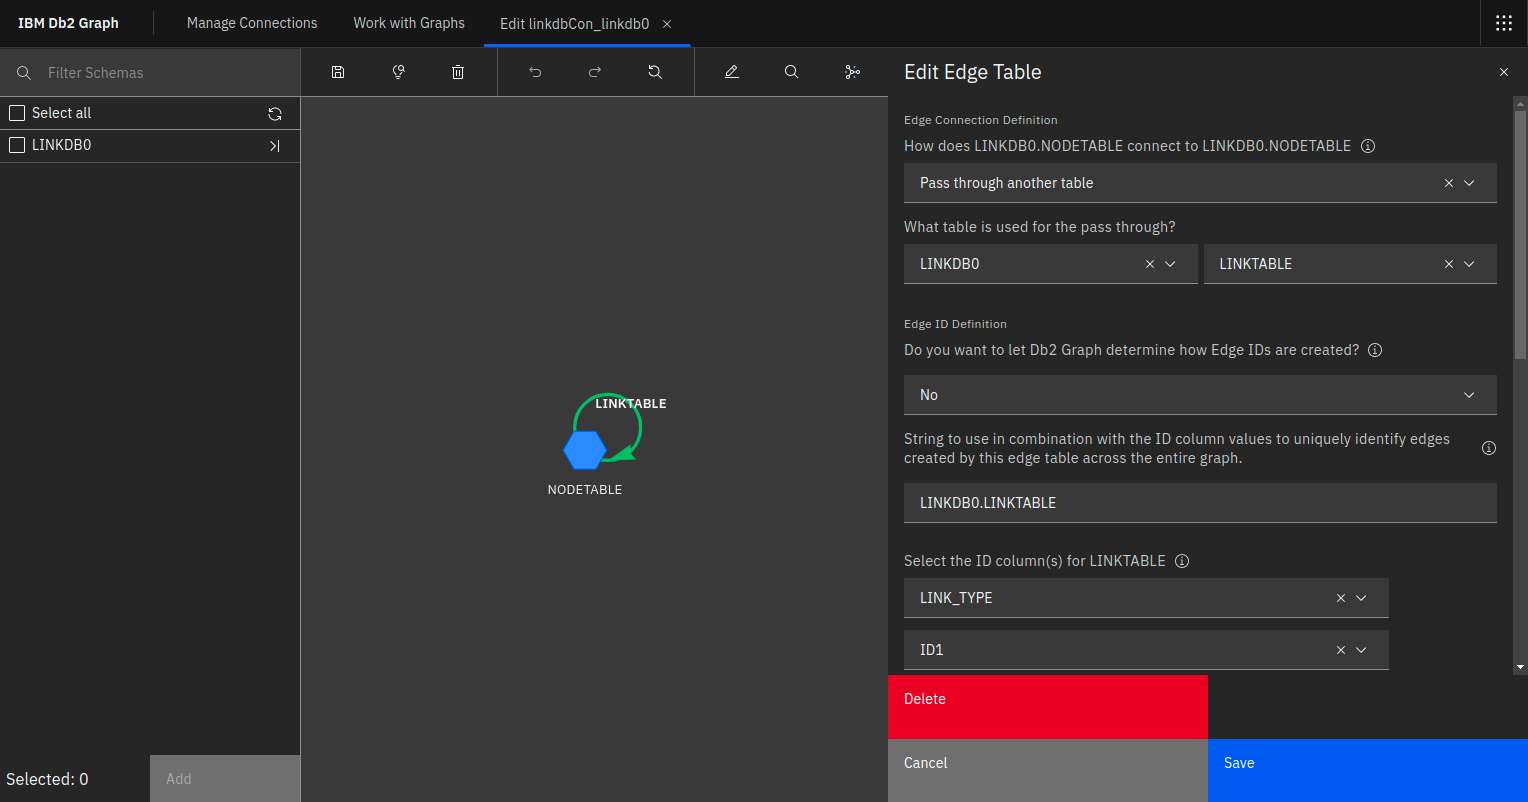
\includegraphics[width=\textwidth]{images/db2_graph_editor.png}
    \vspace{0.1em}
    \caption[Db2 Graph UI -- Graph-Modeler]{Db2 Graph UI -- Graph-Modeler zum Anlegen oder Editieren einer Graph-Overlay-Konfiguration}
    \label{fig:db2_graph_ui_editor}
\end{figure}

Für das Erstellen und Anlegen eines Graphen stellt Db2 Graph UI dabei auch einen sogenannten Graph-Modeler bereit \cite{ibm_docs_db2_graph_ui}. In diesem Graph-Modeler kann ein Graphmodell angelegt und bearbeitet werden. So kann beispielsweise eine Graph-Overlay-Konfiguration mit einigen Klicks erstellt oder angepasst werden, wie in \autoref{fig:db2_graph_ui_editor} gezeigt. Das in \autoref{fig:db2_graph_ui_editor} dargestellte Modell spiegelt dabei eine Konfiguration vergleichbar mit \autoref{src:mapping_example} wider. Die visuelle Darstellung bietet den Vorteil, dass die Vertex-Tabellen und Edge-Tabellen sowie deren Zusammenspiel miteinander schneller erfasst werden können. Siehe das blaue Hexagon \texttt{NODETABLE}, welches eine Vertex-Tabelle repräsentiert oder den grünen Pfeil \texttt{LINKTABLE}, der eine Edge-Tabelle abstrahiert in \autoref{fig:db2_graph_ui_editor}.

Zusätzlich zu dem Graph-Modeler bietet Db2 Graph UI auch eine Web-Console an \cite{ibm_docs_db2_graph_ui}. Diese wird auch als Query-Editor bezeichnet \cite{ibm_docs_db2_graph_ui}. Sie kann dazu genutzt werden, Gremlin-Queries an Db2 Graph zu senden, ähnlich wie die Gremlin-Console. Die Web-Console setzt sich dabei allerdings durch ihre weiteren Funktionen von der Gremlin-Console ab. So besitzt diese auch die Fähigkeit, die abgefragten Elemente eines Graphen visuell darzustellen \cite{ibm_docs_db2_graph_ui}. Einerseits verschafft sie dadurch dem Nutzer einen Überblick über die Ergebnisse einer Gremlin-Query wie in \autoref{fig:db2_graph_webconsole}. Anderseits bietet sie somit die Möglichkeit, mit der Ergebnismenge zu interagieren. Diese Interaktion ergibt sich daraus, dass sich abgebildete Knoten und Kanten auch anklicken und verschieben lassen.

\begin{figure}[!ht]
    \centering
    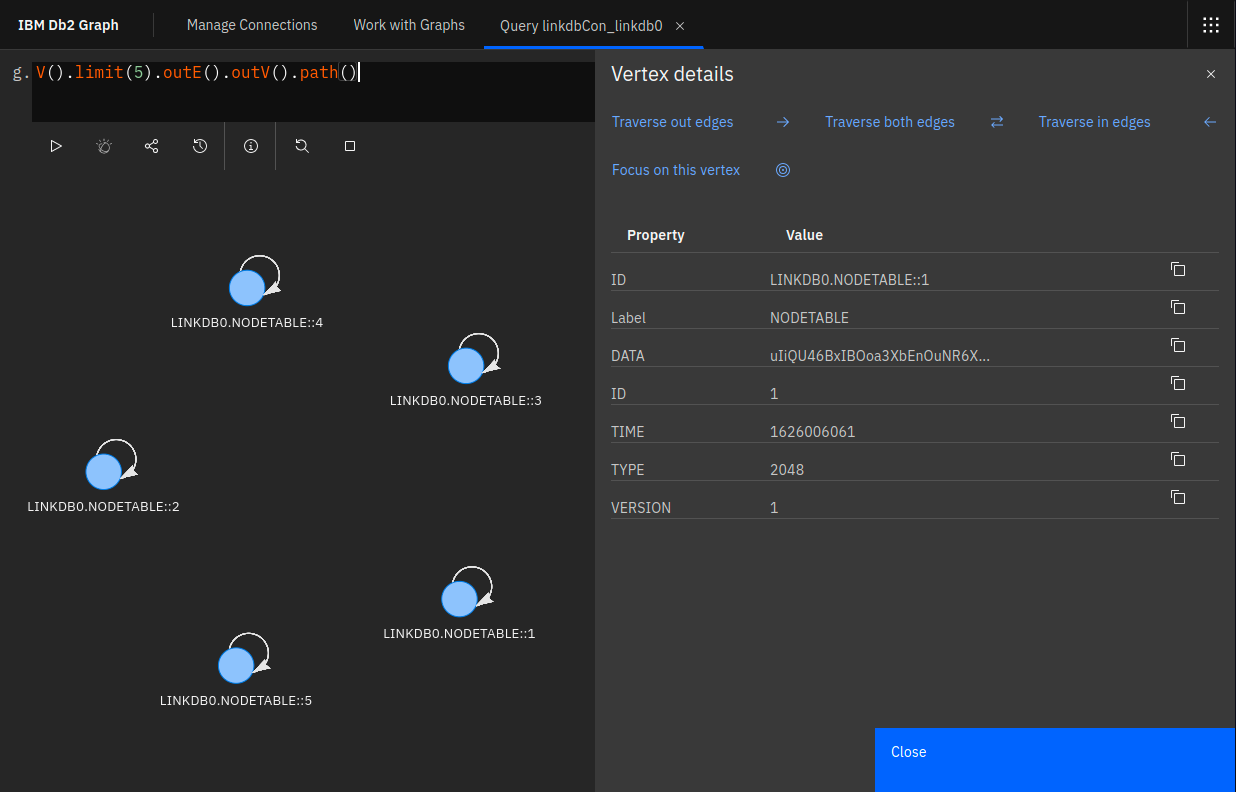
\includegraphics[width=\textwidth]{images/db2_graph_webconsole.png}
    \vspace{0.1em}
    \caption[Db2 Graph UI -- Web-Console]{Db2 Graph UI -- Web-Console}
    \label{fig:db2_graph_webconsole}
\end{figure}

Der aus Beta 3 bekannte \texttt{manage}-Befehl ist, wie bereits zuvor angesprochen auch in V11.5.6.0 verfügbar \cite{ibm_docs_db2_graph_commands}. Allerdings wurde die Fähigkeiten des Befehls erheblich erweitert. So unterstützt er die neue Form des Session-Managements und Verbindungsaufbaus, die mit V11.5.6.0 in Db2 Graph eingeführt wurde \cite{ibm_docs_db2_graph_commands}. Während in Beta 3 die Interaktion mit Db2 Graph kaum Einschränkungen unterlag, erfordert beispielsweise das Anlegen eines Graphen folgende Schritte bei der Arbeit mit dem \texttt{manage}-Befehl:

\begin{enumerate}
    \item Das Öffnen einer Session -- hier \textit{linkdbS} genannt:\\
    \texttt{docker exec -it db2graph manage openSession linkdbS}
    \item Das erstmalige Erstellen einer Connection von Db2 Graph zu Db2 -- hier \textit{linkdbCon} genannt:\\
    \texttt{docker exec -it db2graph manage addConnection linkdbS\break linkdbCon 'Connection to db2 instance with linkdb0 database'\break localhost no 50000 linkdb0 db2inst1 linkdb}
    \item Das Öffnen der Connection -- hier die zuvor erstellte \textit{linkdbCon}:\\
    \texttt{docker exec -it db2graph manage openConnection linkdbS\break linkdbCon db2inst1 linkdb}
    \item Das Anlegen eines neuen Graphen für ein bestimmtes Datenbankschema -- hier \textit{linkdb0} als Graph und \textit{LINKDB0} als Datenbankschema:\\ 
    \texttt{docker exec -it db2graph manage addGraph linkdbS linkdbCon \break linkdb0 LINKDB0}
\end{enumerate}

Konträr zu diesem Ablauf musste bei Db2 Graph Beta 3 lediglich der kurze Dialog, der auf \code{docker exec -it db2graph manage add} folgt, ausgefüllt werden. Darüber hinaus gilt es auch zu erwähnen, dass Db2 Graph UI ebenfalls eine Connection anlegen und öffnen muss, bevor ein Graph-Modell mit dem Graph-Modeler angelegt werden kann \cite{ibm_docs_db2_graph_ui}. Auf das Öffnen einer Session kann jedoch verzichtet werden, da dies von der Weboberfläche automatisch ohne Einbindung des Nutzers erfolgt.

Eine weitere Neuerung, die Einzug in V11.5.6.0 gehalten hat, stellt die Tatsache dar, dass das Graph-Modell eines angelegten Graphen immer auch in die Db2-Datenbank geschrieben wird \cite{ibm_docs_privileges}. Zuvor wurde die Mapping-Konfiguration ausschließlich in Db2 Graph gehalten. Db2 Graph V11.5.6.0 schreibt hingegen ein erstelltes Graph-Modell in die Tabelle \texttt{IBMGRAPH.IBMGRAPHMODEL} einer Db2-Datenbank, welche die Vertex- und Edge-Tabellen des Graph-Modells beinhaltet. 

\subsection{Zusammenfassung}

Bei Db2 Graph handelt es sich um eine Grapherweiterung, die genutzt werden kann, um Graphanfragen an eine relationale Datenbank zu stellen. Um diese Aufgabe zu erfüllen, nutzt sie eine Mapping-Konfiguration. Diese Mapping-Konfiguration beschreibt die Topologie eines Graphen. Dabei regelt sie, welche Tabellen einer Db2-Datenbank Teil des Graphen sind und welche Rolle sie im Graphen einnehmen.

Anhand dieser Topologieinformationen und einer Gremlin-Query erzeugt Db2 Graph SQL-Code. Dieser wird anschließend an eine Db2-Instanz gesendet. Die im Anschluss daran von Db2 an Db2 Graph gesendete Ergebnismenge wird schließlich von Db2 Graph aufbereitet und als Antwort auf die Gremlin-Query weitergegeben. 

Um als Grapherweiterung bei diesem Prozess eine möglichst hohe Performance und geringe Ressourcenauslastung aufzuweisen, beherrscht Db2 Graph eine Vielzahl an Optimierungen. 

Im Rahmen dieser Arbeit werden zwei verschiedene Versionen von Db2 Graph behandelt. Die ältere Variante Beta 3 und die neue Variante V11.5.6.0. Die beiden Versionen unterscheiden sich dabei hauptsächlich in den folgenden drei Punkten:

\begin{itemize}
    \item \textit{Optimierung}\\
    Die Optimierung von Db2 Graph ist in V11.5.6.0 weiter fortgeschritten als in Beta 3. 
    \item \textit{Usability}\\
    Die mit V11.5.6.0 eingeführte Db2 Graph UI erleichtert den Umgang und die Einrichtung von Db2 Graph erheblich. 
    \item \textit{Session- und Connection-Management}\\
    Das in V11.5.6.0 eingeführte Session- und Connection-Management verkompliziert die Interaktion mit Db2 Graph, im Vergleich zu Beta 3.
\end{itemize}